\section{Introduzione}
L'applicazione \texttt{ltspice2circuitikz} permette di convertire un file proveniente dal simulatore LTSpice (file .asc) in un documento contenente il codice latex che rappresenta il circuito simulato tramite l'utilizzo del package \texttt{CircuiTikz} e di generare un file pdf, creato grazie all'applicativo \texttt{pdflatex}, che contiene una rappresentazione del circuito. Inoltre, fornisce una versione formattata correttamente del file .asc in ingresso, nel caso in cui l'utente modifichi manualmente il file prodotto dal simulatore.
\section{Installazione}
L'applicazione attualmente è disponibile solo per il sistema operativo Windows. Per installare l'applicazione è sufficiente decomprimere la cartella compressa \textit{ltspice2circuitikz app.zip}. Una volta decompressa, il contenuto della cartella è il seguente (figura \ref{fig:contenuto}):
\begin{figure}[h!]
	\centering
	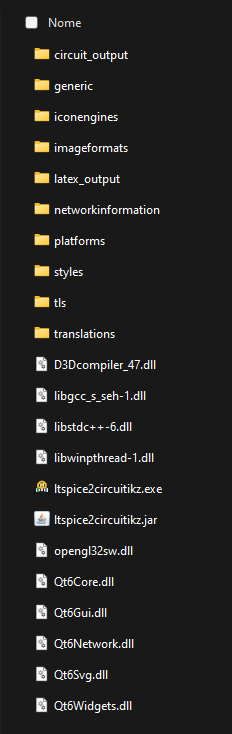
\includegraphics[width=0.25\textwidth]{./ImageFiles/contenuto.png}
	\caption{Contenuto della cartella \textit{ltspice2circuitikz app.zip}.}
	\label{fig:contenuto}
\end{figure}

\noindent
L'applicazione è stata realizzata utilizzando le librerie Qt e l'ambiente di sviluppo Qt IDE. L'utente non deve modificare i file contenuti nella cartella decompressa poiché essi sono necessari al corretto funzionamento dell'applicazione. Invece, il componente che si occupa di eseguire la verifica e la traduzione è stato realizzato in Java. Per il corretto funzionamento dell'applicazione è necessario che sul PC sia installato Java. Inoltre, è necessario avere installato MikTek per la generazione del file PDF a partire dal documento Latex. Per lanciare l'applicazione è sufficiente cliccare due volte sul file \textit{ltspice2circuitikz.exe}.
\section{Funzionalità}
L'applicazione \textit{ltspice2circuitikz} permette di convertire i circuiti generati con il simulatore LTSpice in documenti latex che utilizzano il package \textit{CircuiTikz} per disegnare il circuito in questione. In figura \ref{fig:schema} sono mostrati i file di input e output dell'applicazione. 
\begin{figure}[h!]
	\centering
	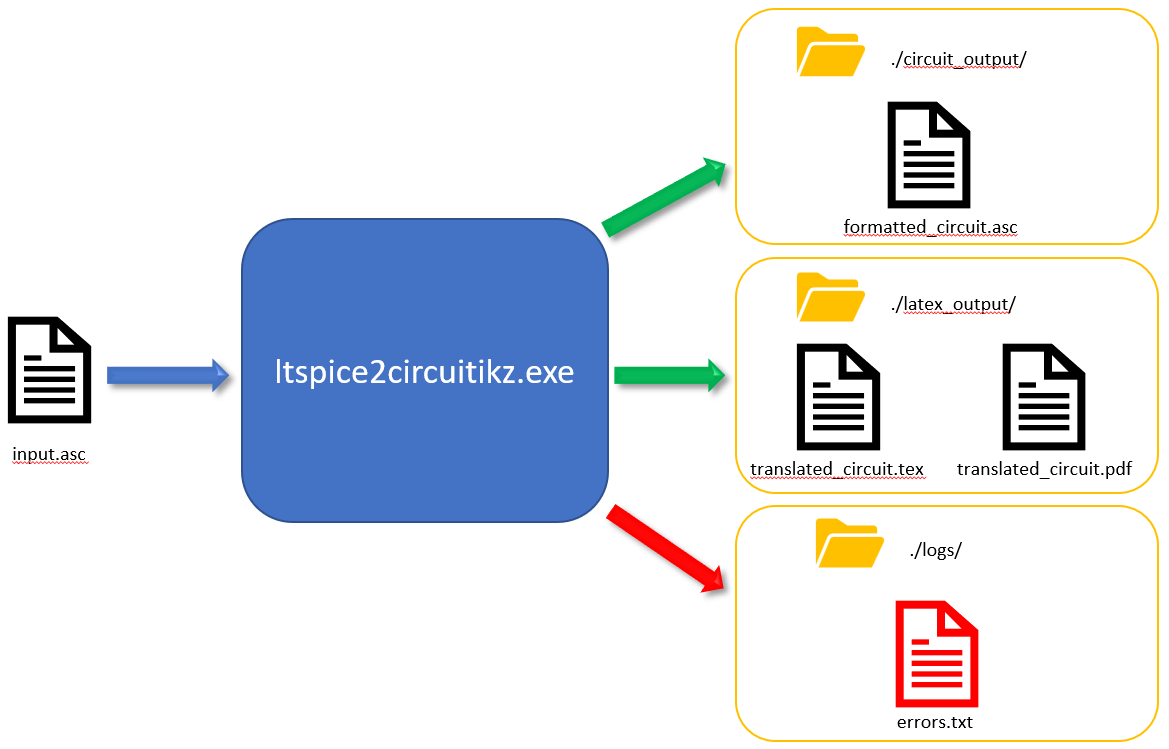
\includegraphics[width=0.8\textwidth]{./ImageFiles/schema funzionamento.png}
	\caption{File in input e output dall'applicazione.}
	\label{fig:schema}
\end{figure}

\noindent
Dopo aver generato un file con estensione .asc tramite il simulatore LTSpice, è possibile importare il file nell'applicazione per la generazione della rappresentazione del circuito in latex. L'applicazione \textit{ltspice2circuitikz} analizza il file in ingresso controllando eventuali errori lessicali, sintattici  e semantici. Nel caso in cui non siano presenti errori, viene eseguita la traduzione e vengono generati tre file:
\begin{itemize}
	\item \textit{translated\_circuit.tex}: contiene il codice latex che permetterà di generare la rappresentazione del circuito in un file pdf;
	\item \textit{translated\_circuit.pdf}: è il file pdf generato a partire dal file latex; 
	\item \textit{formatted\_circuit.tex}: contiene il testo del file .asc formattato in modo corretto, in cui ogni token è separato da uno spazio e ogni parole chiave è all'inizio di una nuova riga.
\end{itemize}
Nel caso in cui siano presenti degli errori, essi sono mostrati nella console dell'applicazione. Inoltre, gli errori generati vengono salvati in un file \textit{errors.txt} all'interno della cartella \texttt{./logs/}.
Durante la generazione del file latex, vengono tenute in considerazione le dimensioni del circuito che si vuole generare e, nel caso in cui la larghezza superi l'altezza, il circuito generato verrà ruotato automaticamente per sfruttare meglio lo spazio disponibile. Nella documento \textit{Documentazione Tecnica} sono riportati tutti i dettagli sulla lettura del file in ingresso e sul processo di traduzione.

\clearpage

\section{Grammatica file .asc}
Nel normale utilizzo dell'applicazione \textit{ltspice2circuitikz} non è necessario conoscere la grammatica del file .asc in quanto tale file viene generato dal programma LTSpice. Tuttavia, per completezza, vengono riportate di seguito le regole della grammatica ricavata dall'analisi dei file asc prodotti dal simulatore. È importante notare che la grammatica è stata ricavata tramite un processo di \textit{reverse engineering} e pertanto potrebbe non essere completa.
\begin{itemize}
	\item \texttt{Version 4}: tutti i file iniziano con la seguente regola. L'applicazione è in grado di gestire solo la versione 4, che è quella attualmente usata dall'ultima versione di LTSpice;
	\item \texttt{SHEET int width height}: il primo intero rappresenta il numero del foglio, i due interi successivi rappresentano le dimensioni di tale foglio;
	\item \texttt{WIRE x1 y1 x2 y2}: rappresenta un filo di collegamento, seguito dalle coordinate x1, y1 ed x2, y2 dei capi del filo;
	\item \texttt{FLAG x y content}: rappresenta posizione e contenuto di eventuali label associati ad un collegamento. Se il contenuto è 0, allora si indica la massa del circuito;
	\item \texttt{SYMBOL type x y rotation}: rappresenta un componente. Le tipologie di componenti riconosciute dall'applicazione sono \textit{res}, \textit{cap}, \textit{polcap} \textit{ind}, \textit{diode} e \textit{voltage}. Il campo rotazione può contenere i seguenti valori: \textit{R0}, \textit{R90}, \textit{R180}, \textit{R270}, \textit{M0}, \textit{M90}, \textit{M180} e \textit{M270}. La lettera M indica che il componente oltre ad essere ruotato è anche specchiato;
	\item \texttt{SYMATTR type \textlangle ...\textrangle}: permette di specificare eventuali attributi riferiti ad un componente, come per esempio il nome, il valore o altri parametri;
	\item \texttt{WINDOW number x y pos size}: indica la posizione di una label associata ad un componente e la sua dimensione;
	\item \texttt{IOPIN x y \textlangle In/Out/BiDir\textrangle}: indicano una label di ingresso o uscita nel circuito.
\end{itemize}
Queste regole sono state utilizzate per generare la grammatica alla base del lexer e del parser realizzato per generare l'applicazione. La grammatica completa è riportata nella \textit{Documentazione Tecnica}

\clearpage

\section{Esempio di utilizzo}
Di seguito viene mostrato come utilizzare l'applicazione \textit{ltspice2circuitikz}. 
\begin{enumerate}
	\item Aprire l'applicazione \textit{ltspice2circuitikz} cliccando due volte l'eseguibile \textit{ltspice2circuitikz.exe}. Si aprirà una schermata come quella mostrata in figura \ref{fig:punto_1}.
	\begin{figure}[h!]
		\centering
		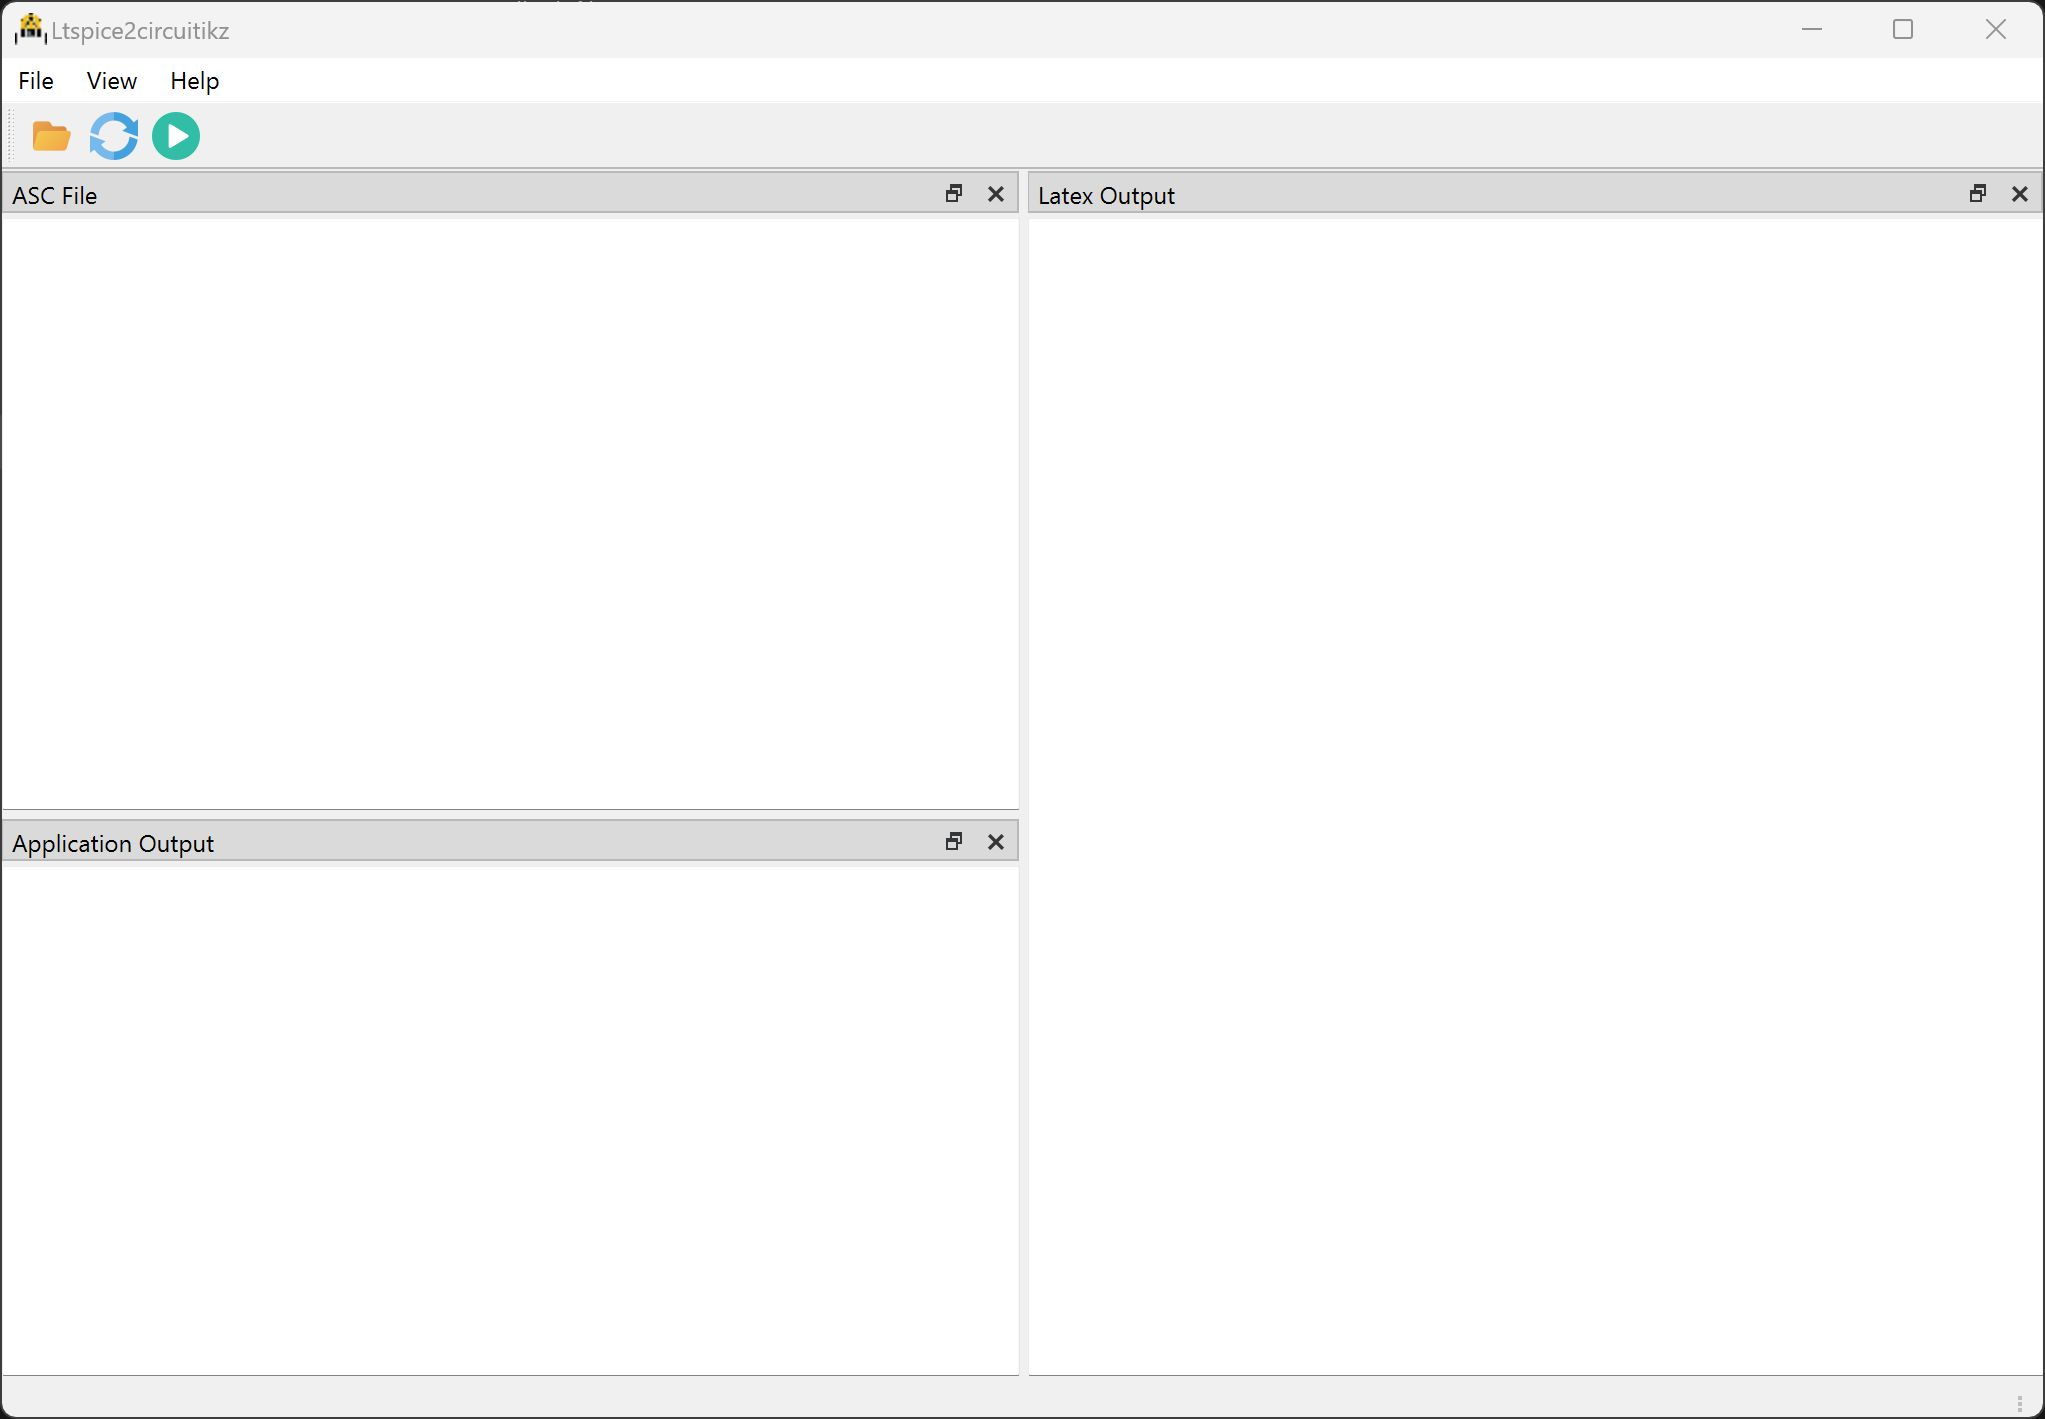
\includegraphics[width=0.7\textwidth]{./ImageFiles/mainview.png}
		\caption{Schermata principale dell'applicazione.}
		\label{fig:punto_1}
	\end{figure}
	\item Cliccare l'icona \textit{"Open File"} e selezionare un file .asc da aprire. Una volta selezionato il file, il suo contenuto verrà mostrato nella finestra in alto a sinistra (figura \ref{fig:punto_2}). Il contenuto del file non può essere modificato dall'applicazione ma deve essere modificato da un tool esterno. Nel caso venga modificato è possibile ricaricare il file premendo l'icona di \textit{"Refresh"}.
	\begin{figure}[h!]
		\centering
		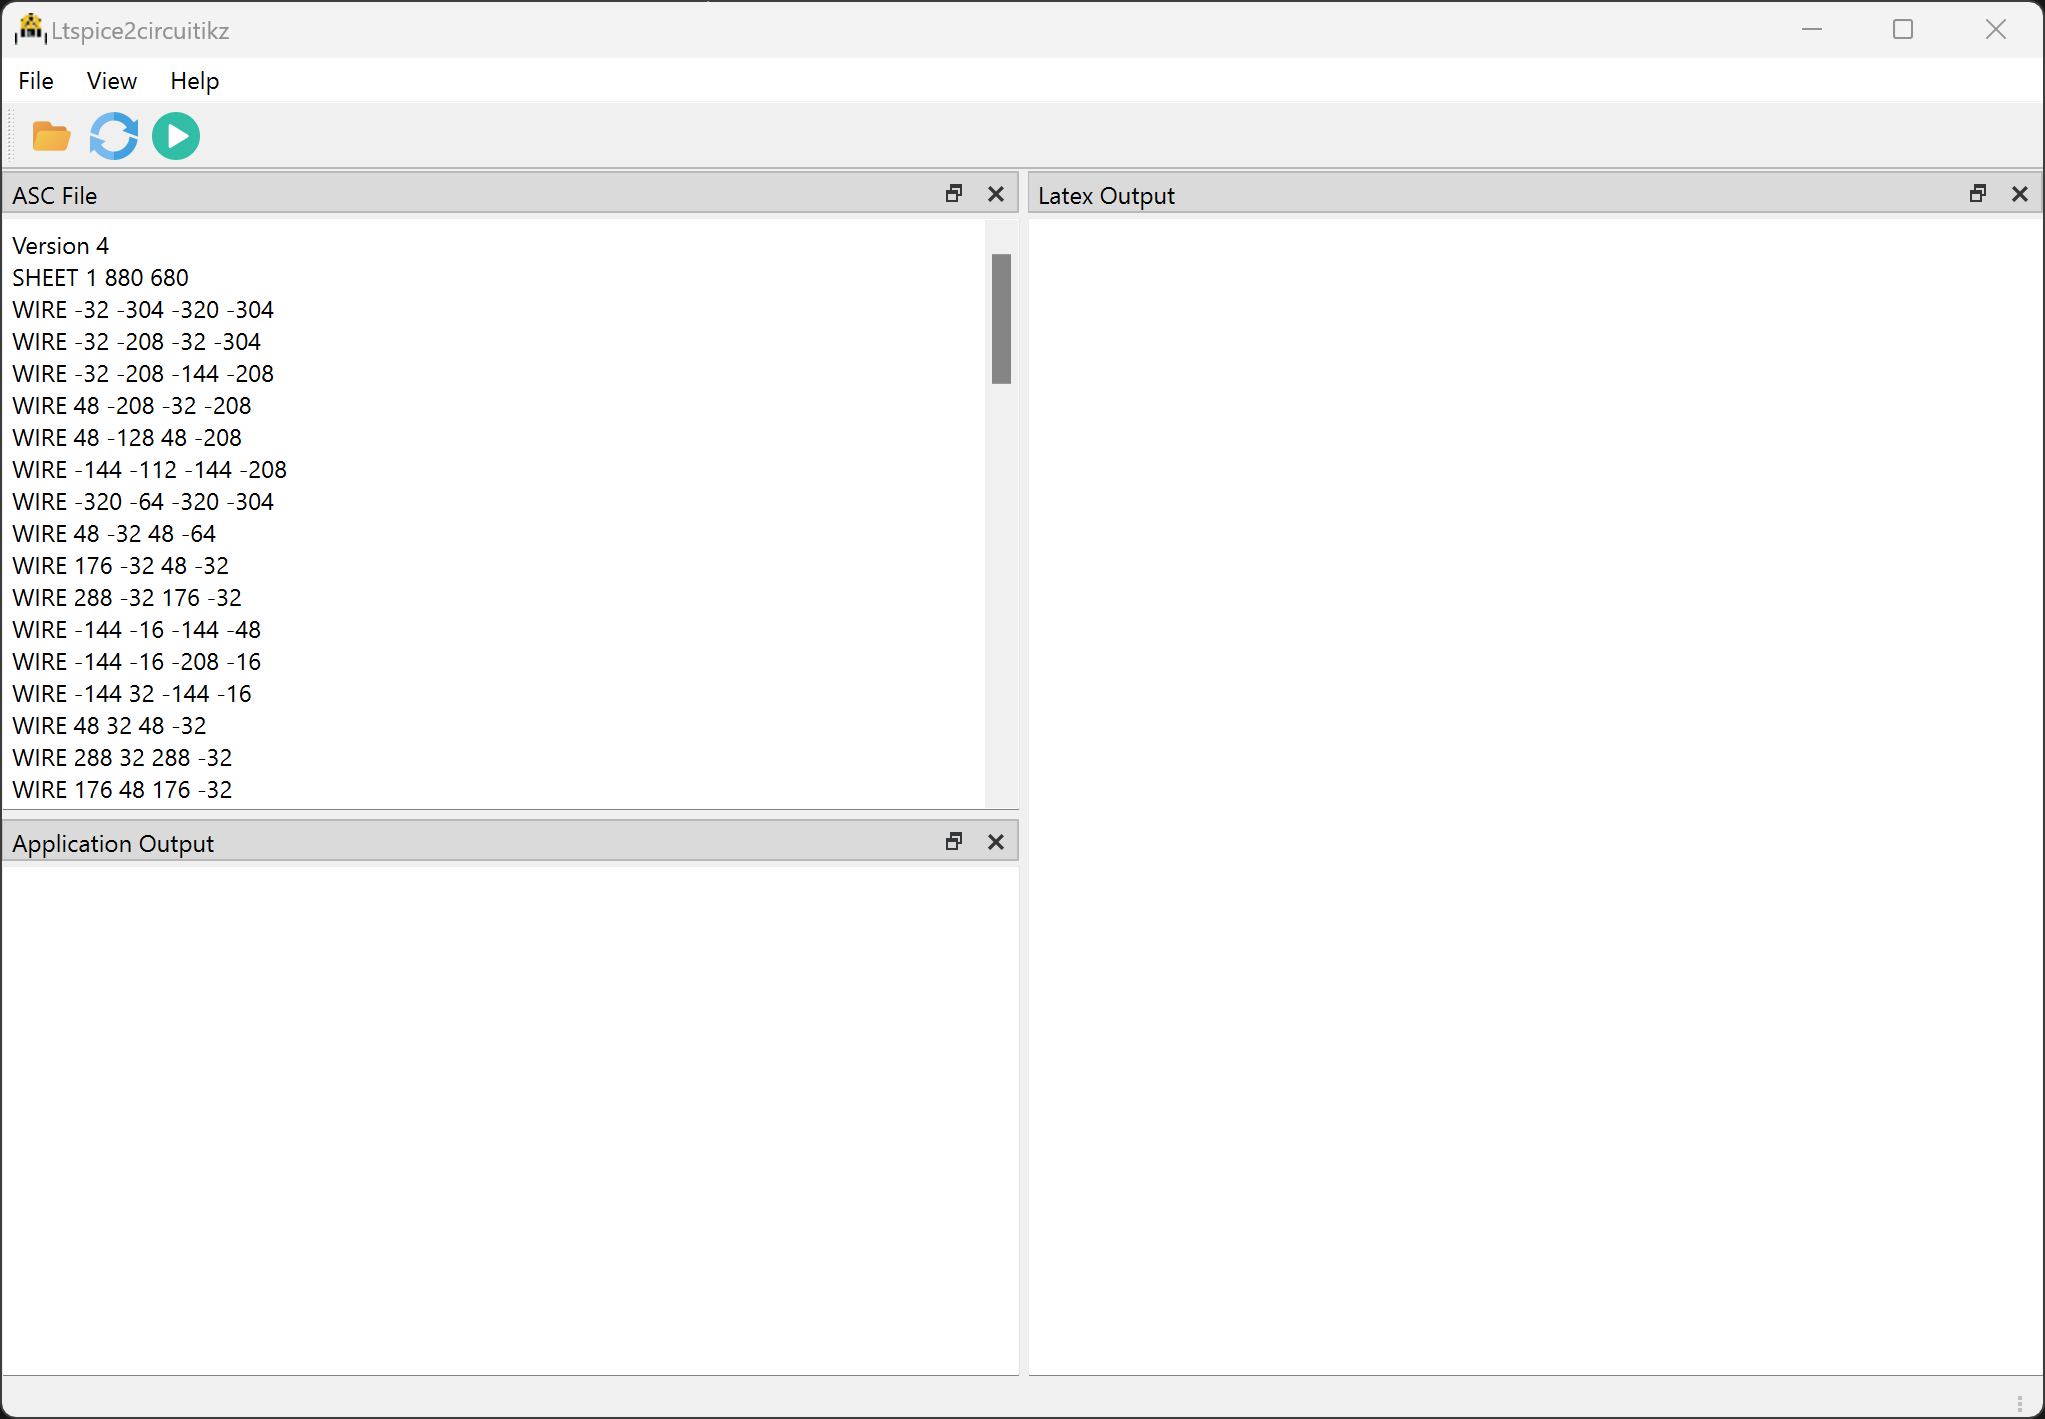
\includegraphics[width=0.7\textwidth]{./ImageFiles/file aperto.png}
		\caption{Schermata che mostra il file aperto.}
		\label{fig:punto_2}
	\end{figure}
	\newpage
	\item Premere il pulsante verde \textit{"Run"} per lanciare il processo di conversione. Se non ci sono errori, viene mostrato un messaggio verde nell'\textit{Application Output} e viene caricato il contenuto del file latex nella colonna di destra (figura \ref{fig:punto_3}). Inoltre, viene aperto il file pdf contenente il circuito generato. Se si vuole mostrare anche il file formattato in modo corretto, è sufficiente selezionare la voce \textit{"Formatted ASC File"} nel menù \textit{"View"}.
	\begin{figure}[h!]
		\centering
		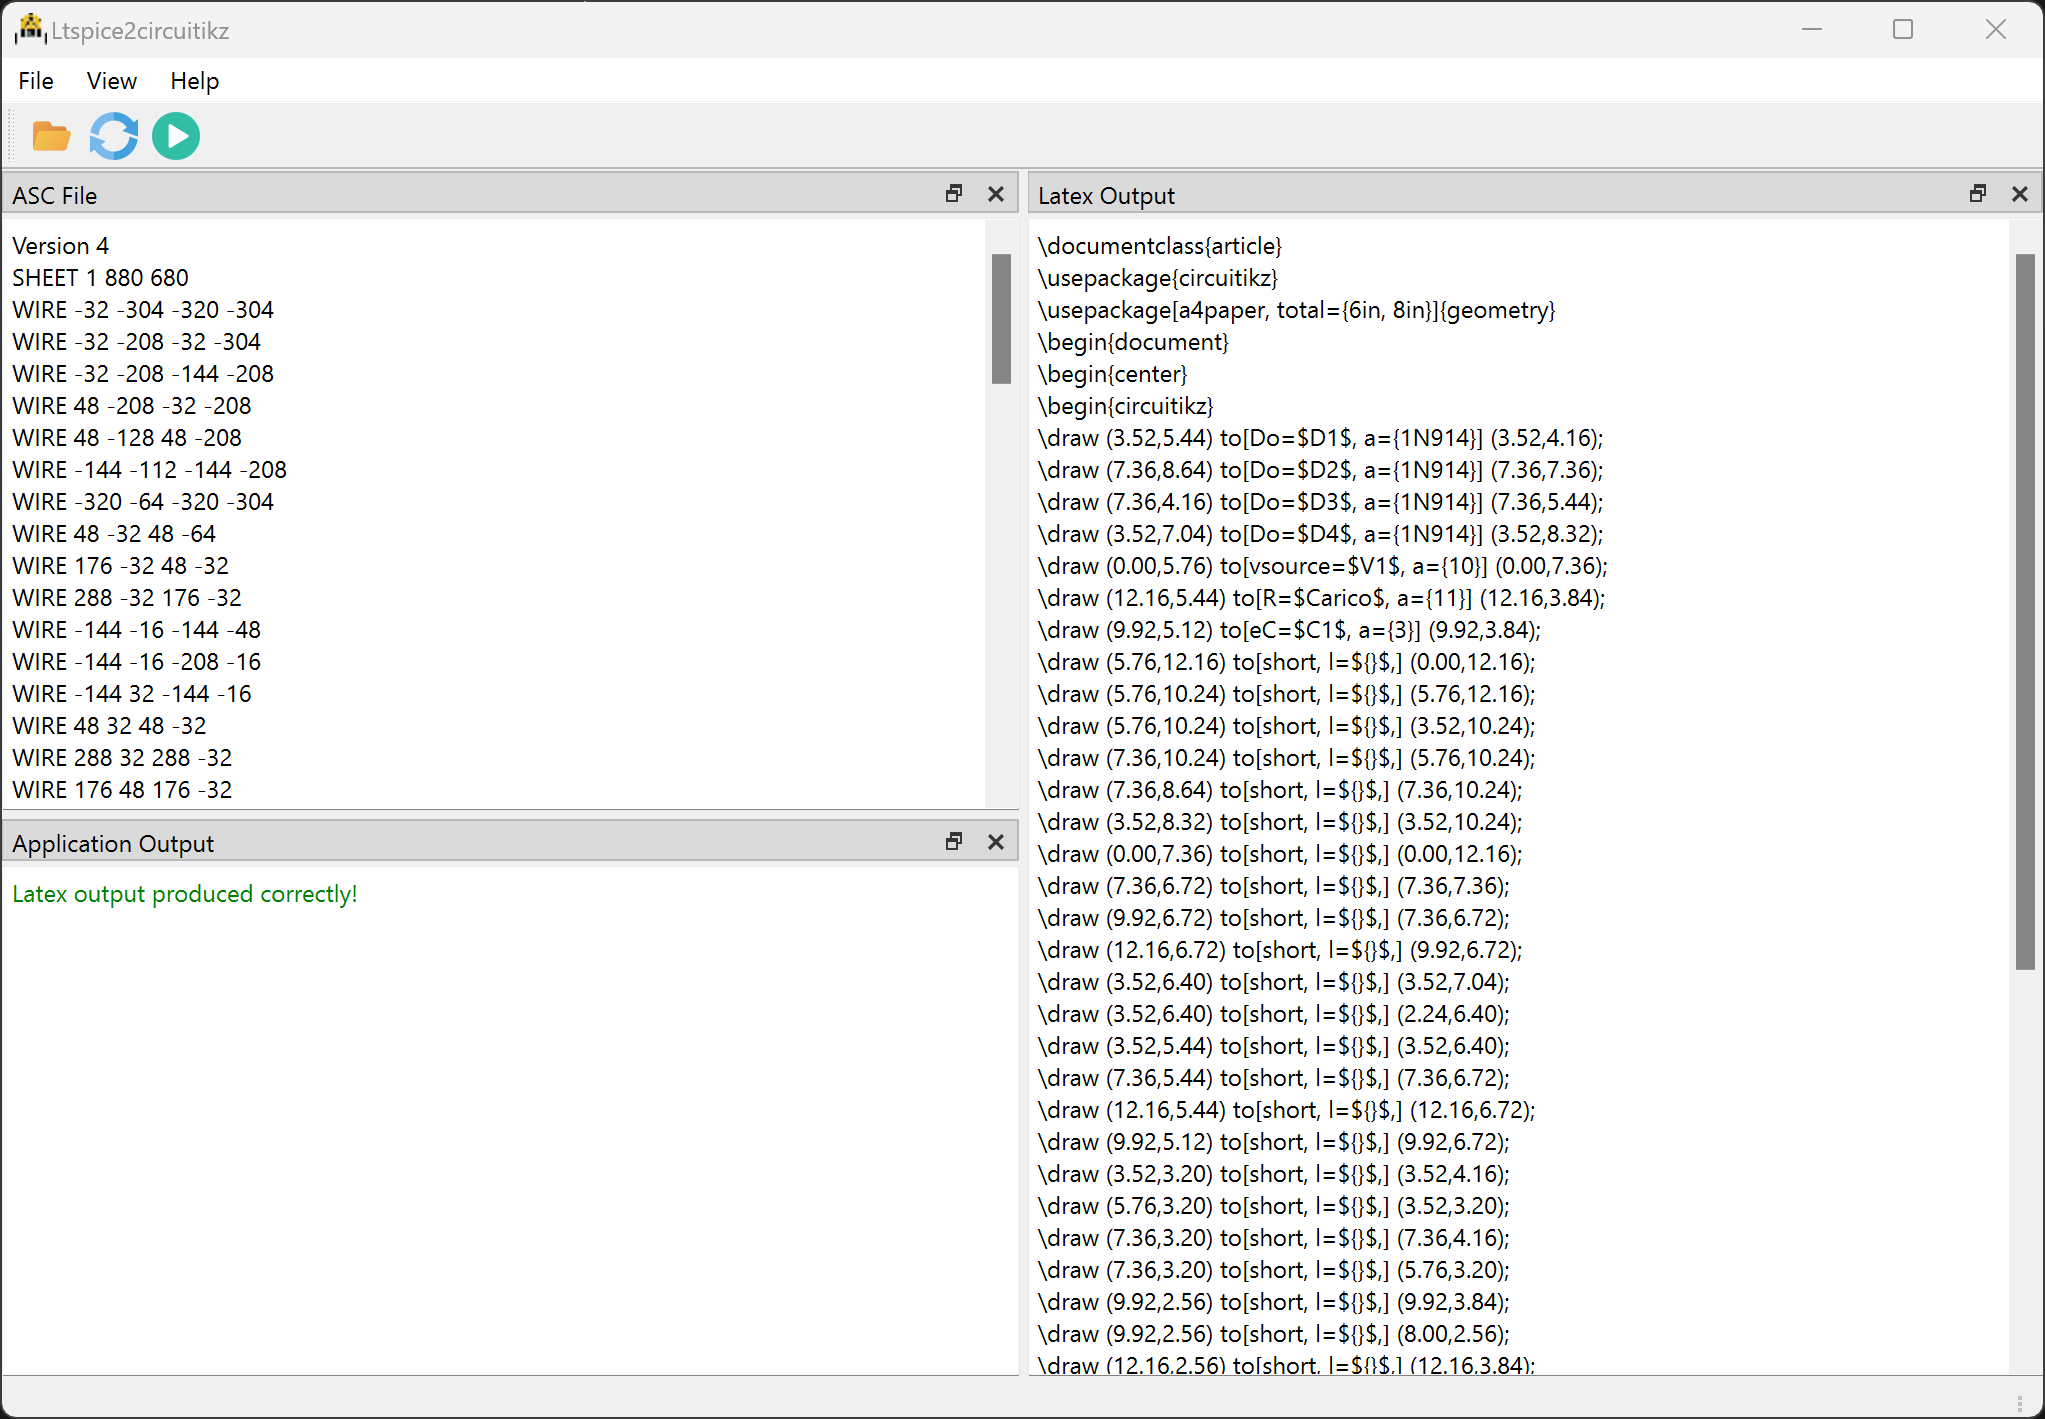
\includegraphics[width=0.7\textwidth]{./ImageFiles/run con successo.png}
		\caption{Processo eseguito con successo.}
		\label{fig:punto_3}
	\end{figure}
	\item Nel caso in cui ci siano errori semantici o sintattici, il processo si interrompe e nell'\textit{Application Output} vengono mostrati gli errori (figura \ref{fig:punto_4}).
	\begin{figure}[h!]
		\centering
		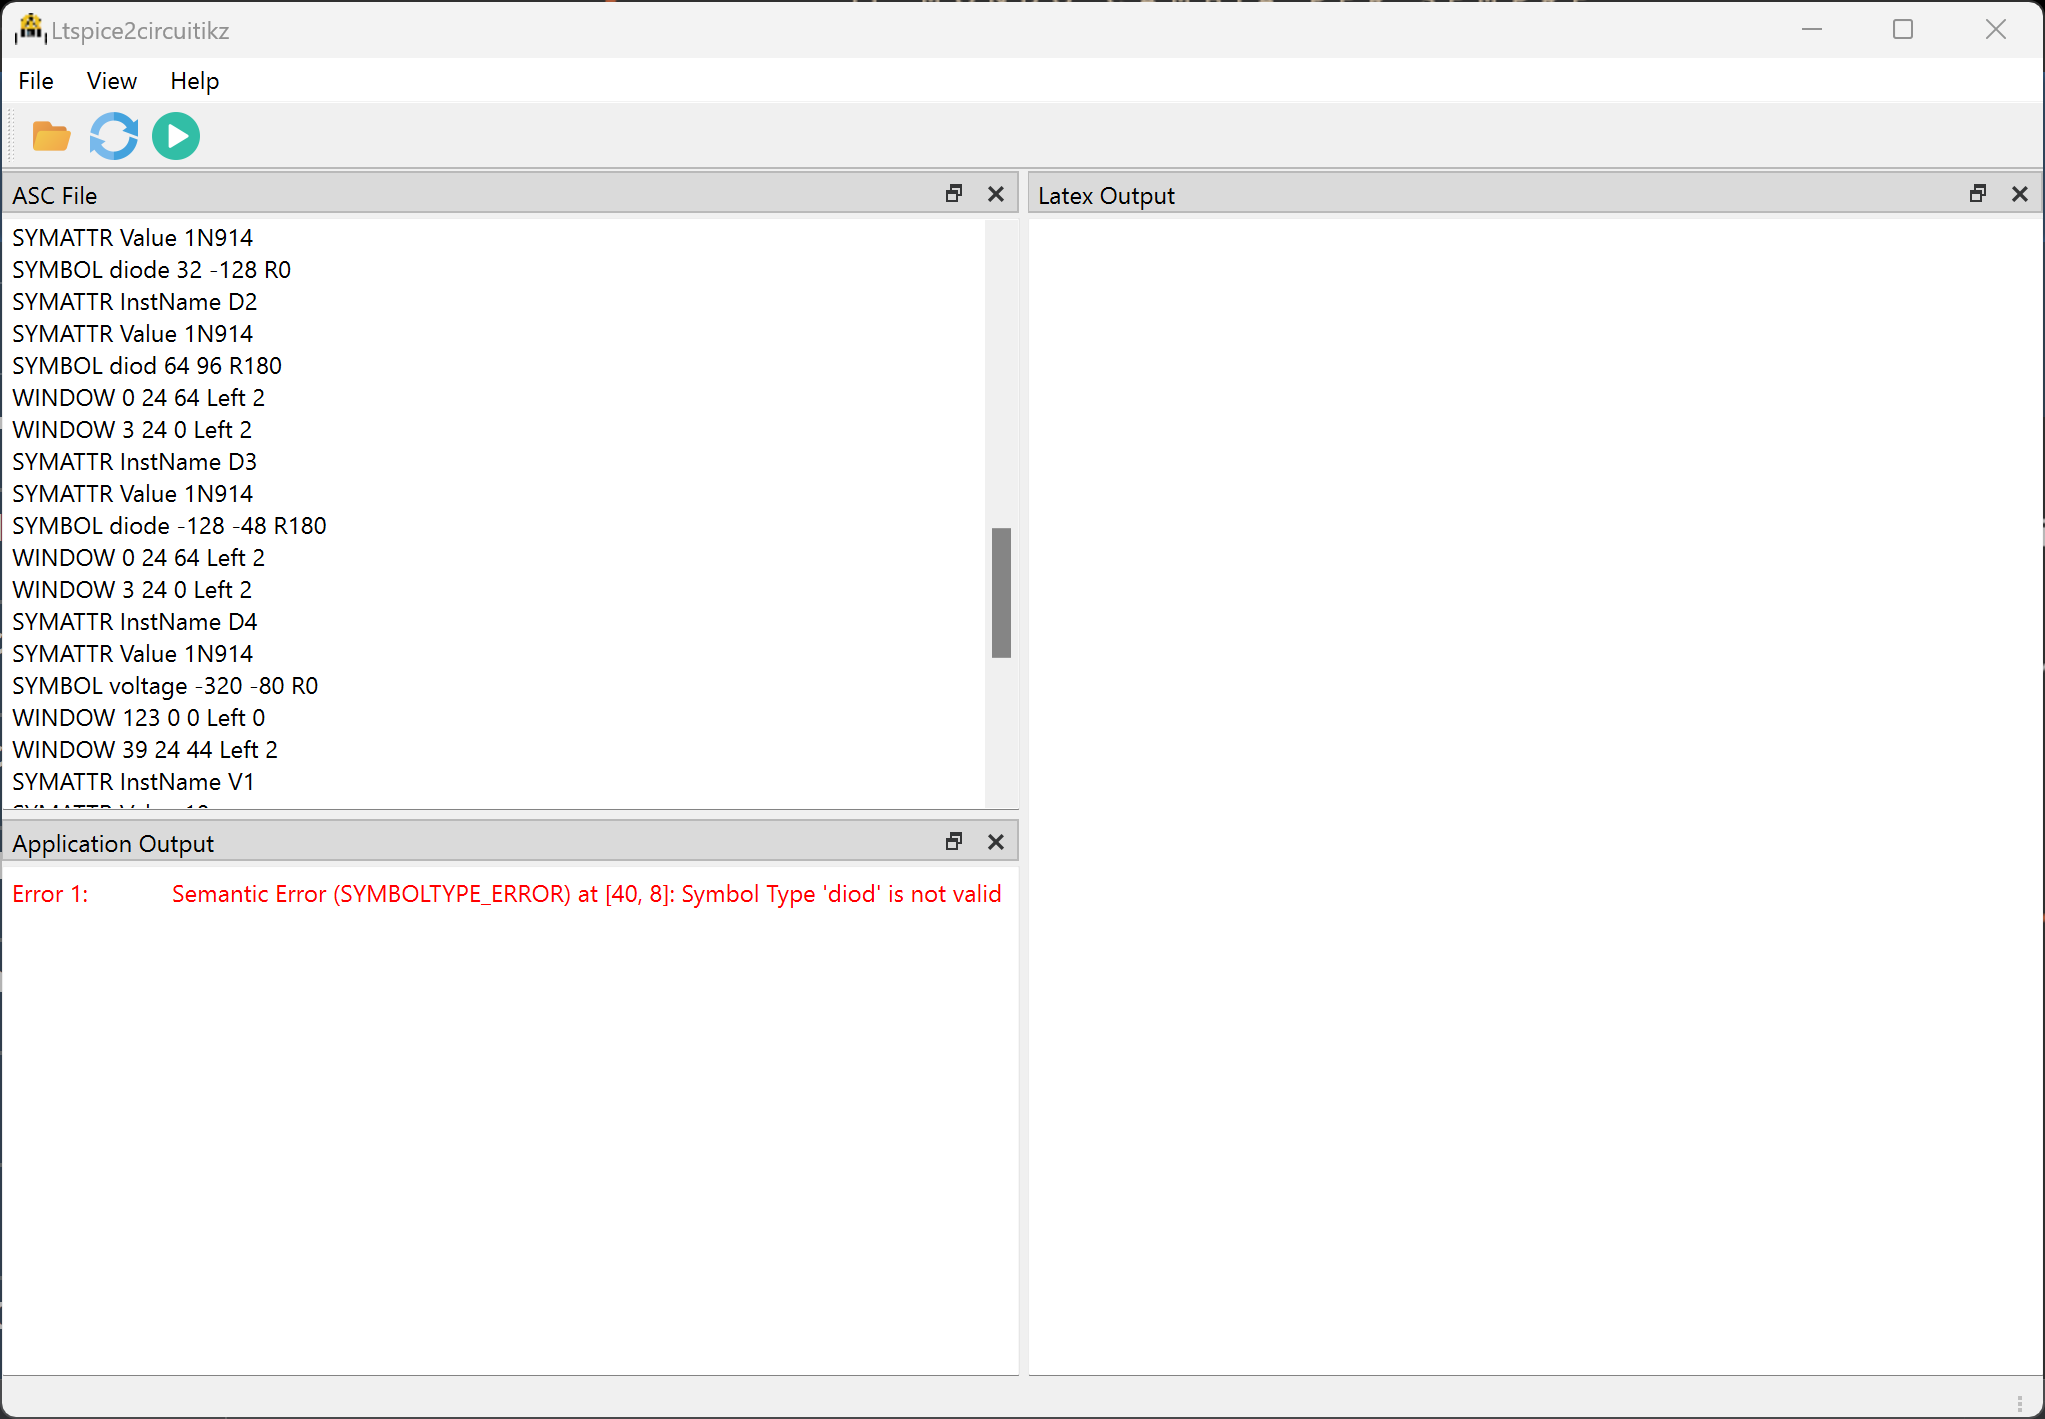
\includegraphics[width=0.7\textwidth]{./ImageFiles/semantic error.png}
		\caption{Errori semantici.}
		\label{fig:punto_4}
	\end{figure}
\end{enumerate}




